\documentclass[draft,grl]{agutexSI2018}
\usepackage{apacite}

%%%%%%%%%%%%%%%%%%%%%%%%%%%%%%%%%%%%%%%%%%%%%%%%%%%%%%%%%%%%%%%%%%%%%%%%%
%
%  SUPPORTING INFORMATION TEMPLATE
%
%% ------------------------------------------------------------------------ %%
%
%
%Please use this template when formatting and submitting your Supporting Information.

%This template serves as both a “table of contents” for the supporting information for your article and as a summary of files.
%
%
%OVERVIEW
%
%Please note that all supporting information will be peer reviewed with your manuscript.
%In general, the purpose of the supporting information is to enable authors to provide and archive auxiliary information such as data %tables, method information, figures, video, or computer software, in digital formats so that other scientists can use it.
%The key criteria are that the data:
% 1. supplement the main scientific conclusions of the paper but are not essential to the conclusions (with the exception of
%    including %data so the experiment can be reproducible);
% 2. are likely to be usable or used by other scientists working in the field;
% 3. are described with sufficient precision that other scientists can understand them, and
% 4. are not exe files.
%
%USING THIS TEMPLATE
%
%***All references should be included in the reference list of the main paper so that they can be indexed, linked, and counted as citations.  The reference section does not count toward length limits.
%
%All Supporting text and figures should be included in this document. Insert supporting information content into each appropriate section of the template. %Figures and tables should appear above each caption.  To add additional captions, simply copy and paste each sample caption as needed.

%Tables may be included, but can also be uploaded separately, especially if they are larger than 1 page, or if necessary for retaining table formatting. Data sets, large tables, movie files, and audio files should be uploaded separately, following AGU naming conventions. Include their captions in this document and list the file name with the caption. You will be prompted to upload these files on the Upload Files tab during the submission process, using file type “Supporting Information (SI)”

%IMPORTANT NOTE ON FIGURES AND TABLES
% Placeholders for figures and tables appear after the \end{article} command, after references.
% DO NOT USE \psfrag or \subfigure commands.
%
%  Uncomment the following command to include .eps files
\usepackage[dvips]{graphicx}
%
%  Uncomment the following command to allow illustrations to print
%   when using Draft:
\setkeys{Gin}{draft=false}
%
% Substitute one of the following for [dvips] above
% if you are using a different driver program and want to
% proof your illustrations on your machine:
%
% [xdvi], [dvipdf], [dvipsone], [dviwindo], [emtex], [dviwin],
% [pctexps],  [pctexwin],  [pctexhp],  [pctex32], [truetex], [tcidvi],
% [oztex], [textures]
%
%
%% ------------------------------------------------------------------------ %%
%
%  ENTER PREAMBLE
%
%% ------------------------------------------------------------------------ %%

% Author names in capital letters:
%\authorrunninghead{BALES ET AL.}

% Shorter version of title entered in capital letters:
%\titlerunninghead{SHORT TITLE}

%Corresponding author mailing address and e-mail address:
%\authoraddr{Corresponding author: A. B. Smith,
%Department of Hydrology and Water Resources, University of
%Arizona, Harshbarger Building 11, Tucson, AZ 85721, USA.
%(a.b.smith@hwr.arizona.edu)}

\begin{document}

%% ------------------------------------------------------------------------ %%
%
%  TITLE
%
%% ------------------------------------------------------------------------ %%

%\includegraphics{agu_pubart-white_reduced.eps}


\title{Supporting Information for ``The importance of ice sheet growth and retreat on magmatism and mantle CO$_2$ flux''}


\authors{John J.~Armitage\affil{1}, David J.~Ferguson\affil{2}, Kenni D.~Petersen\affil{3}, and Timothy T.~Creyts\affil{4}}

\affiliation{1}{Dynamique des Fluides G{\'e}ologiques, Institut de Physique du Globe de Paris, Paris, France}
\affiliation{2}{School of Earth and Environment, University of Leeds, Leeds, U.K.}
\affiliation{3}{Department of Geoscience, University of Aarhus, Aarhus, Denmark}
\affiliation{4}{Lamont-Doherty Earth Observatory, Columbia University, U.S.A}


\begin{article}

\noindent\textbf{Contents of this file}
\begin{enumerate}
\item Text S1 to S3
\item Figures S1 to S3
\end{enumerate}
\noindent\textbf{Additional Supporting Information (Files uploaded separately)}
\begin{enumerate}
\item Table S1
\item Data Set S1
\end{enumerate}

\clearpage

\noindent\textbf{Introduction}
We develop a model of lithosphere flexure due to the glaciation and deglaciation that is coupled to melting within the asthenosphere and the subsequent transport of that melt to the surface. In order to drive the model we also must estimate past Icelandic ice sheet thickness (see Text S1 below). What follows is a description of these two models.

\noindent\textbf{Text S1.}

\noindent\textit{Generating an Ice sheet History}

Our goal is to create realizations of ice loading over the Iceland rift zone. The ice volume history of Iceland through the entire last glacial period is fragmentary, and poorly constrained prior to the Last Glacial Maximum (26-110\,ka) \citep{geirsdottir-2011}.  This lack of information is a result of the growth of the ice sheet to the LGM ($\sim$19-26.5\,ka) \citep{geirsdottir-2011,clark-etal-2009}, because it reworks prior deposits and remobilizes sediments, obscuring the earlier record \citep{andrews-2008}. Additionally, we are mainly interested in the loading history and less concerned with the extent, glacial features, or ice rafted debris, that are specific to the extent and configuration of the Icelandic Ice Sheet. We therefore only require a realization from which to run the melting model. Hence we believe simplified ice sheet history is sufficient to understand the magmatism in Iceland. 

We develop a simple method of reconstructing the volume using published ice sheet model results. We use the results of \citet{patton-etal-2017} to identify the ice thickness over the rift zone. Their model results are designed to understand the configuration of the ice sheet during the deglaciation. This time period is also the best constrained in terms of the sea level history \citep{spratt-2016,andersen-etal-2004} and deglacial climate \citep{lambeck-2001}. Recognizing that the \citet{patton-etal-2017} model is driven by the NGRIP climate record \citep{lambeck-2001} and also that the volume of ice sheets is also contained in sea level histories \citep{spratt-2016}, we use these to constrain ice sheet history prior to the LGM.

We create rift zone loading histories that extend back through the last glacial to the previous interglacial period. We perform a parametric regression on the rift ice load, the NGRIP $\delta^{18}$O record, and the deglacial sea level record through the deglaciation. We then use the coefficients of the deglacial history to extend the ice sheet load back in time using published sea level records \citep{peltier-2004,pico-etal-2017}.

We regress the ice sheet results against the ice core $\delta^{18}$O \citep{lambeck-2001} and the relative sea level curve \citep{spratt-2016}:
\begin{equation}
v_{ind} = a_{1} \delta_{NGRIP} + a_{2} \Delta\zeta_{esl} + c
\label{eq:1}
\end{equation}
We seek an index for the volume of the Icelandic Ice Sheet $v_{ind}$ by solving for the coefficients $a_{1}$ and $a_{2}$, as well as the offset $c$, where $\delta_{NGRIP}$ is the ice core oxygen isotope record and  $\Delta\zeta_{esl}$ is the relative sea level height. We use the results of \citet{patton-etal-2017} from 10 ka to 23.5\,ka so that $a_{1} = -21.94$, $a_{2} = -4.993$. Figure S1 shows how each of the input time series yields the scaled time series. We then apply these coefficients to the remainder of the NGRIP and sea level histories to get the loading from 120,000 years to the present (Figure S2). Because sea level is not well-constrained through the last glacial period, we utilize three different sea level curves to produce the relative ice sheet volume (Figure S2). We then scale the ice sheet histories to give a maximum ice sheet thickness of 1800\,m. We force the melting model with the two ice sheet histories, the M1 model based on the sea level curve ICE-5G \citep{peltier-2004} and the model M2 based on the sea level curve of \citet{pico-etal-2017}.

\noindent\textbf{Text S2.}

\noindent\textit{Numerical Melting Model Description and Methods}

We solve for the conservation of energy and the vertical percolation of melt within a one-dimensional vertical column. We define a average velocity of the solid and liquid phases \citep{scott-1992},
\begin{equation}
\bar{v} = (1-\phi)v_{s} + \phi v_{l},
\label{eq:2}
\end{equation}
where $\phi$ is porosity, $v_{s}$ is the solid mantle velocity, $v_{l}$ is the melt velocity. All model parameters are listed in Table S1. The change in surface load is assumed to impact the average velocity. We calculate the displacement due to a ice sheet where the change in surface displacement, $w_{0}$, with time is given by \citep{sleep-1976},
\begin{equation}
N\frac{\partial^{4}}{\partial x^{4}} \left(\frac{\partial w_{0}}{\partial t} \right) = \frac{P_{ice}}{\tau_{e}},
\label{eq:3}
\end{equation}
where $N$ is the elastic flexural rigidity, $P_{ice}$ is the load due to the ice sheet, and $\tau_{e}$ is the viscoelastic decay time. The elastic flexural rigidity is given by,
\begin{equation}
N = \frac{E T_{e}}{12(1-\mu^{2})},
\label{eq:4}
\end{equation}
where $E$ is Young's modulus, $T_{e}$ is the effective elastic thickness, and $\mu$ is Poisson's ratio. The viscoelastic decay time is defined as \citep{sleep-1976},
\begin{equation}
\tau_{e} = \frac{3\eta_{s}}{E},
\label{eq:5}
\end{equation}
where $\eta_{s}$ is the viscosity of the lithosphere. Equation \ref{eq:3} is solved using a simple finite element model with linear weighting functions, to solve for $w_{0}$ as a function of time due to the change in surface load. The vertical velocity of the mantle below is then updated by the rate of change in displacement due to the surface load, assuming that the displacement decays with depth as a function of the wavelength (width), $\lambda$, of the ice load \citep{england-etal-1985},
\begin{equation}
w = w_{0} exp\left(-\sqrt{3}\pi \frac{z}{\lambda}\right).
\label{eq:6}
\end{equation}
Therefore the vertical velocity is given by,
\begin{equation}
\bar{v} = u + \frac{\partial w}{\partial t},
\label{eq:7}
\end{equation}
where $u$ is the constant upwelling rate.

The model is then either run as a single upwelling column with a fixed upwelling rate (1D) or we use the steady state solution to the corner flow of mantle hitting a horizontal plain to get create a 2D flow field from which to extract the vertical upwelling rate \citep{silbeck-1975}. In the 1D version the displacement at the centre of the model, $\partial w/\partial t$, is used to perturb the vertical velocity, while in the 2D version we take take a width of displacement from 0 to 80\,km from the centre of extension, and assume melt travels vertically upwards in 1D columns. The displacement at each point from 0 to 80 \,km is used to perturb the vertical velocity from the corner flow solution.

To calculate the vertical flow of melt as function of variations in the decompression rate, the conservation of energy is given by,
\begin{equation}
mL + \frac{\partial T}{\partial t} + \bar{v}\frac{\partial T}{\partial z} - \kappa\frac{\partial^{2} T}{\partial z^{2}} = 0,
\label{eq:8}
\end{equation}
where $m$ is the melt production rate, $L$ is the latent heat of fusion, $T$ is temperature, and $\kappa$ is the thermal diffusion coefficient. The latent heat is given by, $L = T\Delta S/C_{p}$, where $\Delta S$ is the entropy change due to melting and $C_{p}$ is the heat capacity. The conservation of mass for the liquid phase is given by,
\begin{equation}
\frac{\partial \phi}{\partial t} + \frac{\partial}{\partial z}\left(\phi v_{l}\right) = m.
\label{eq:9}
\end{equation}

To relate the solid velocity to the liquid velocity we turn to Darcy's law,
\begin{equation}
\phi\left(v_{l}-v_{s}\right) = \frac{k_{0}\phi^{n}}{\eta_{l}}\left(\Delta\rho g + \frac{\partial P}{\partial z}\right),
\label{eq:10}
\end{equation}
where $k_{0}$ is the permeability coefficient, $n$ is the exponent on the assumed power law relation between permeability and porosity, $\Delta\rho$ is the density difference between melt and the solid mantle, $g$ is gravity, and $P$ is the pore pressure. We simplify equation \ref{eq:10} by assuming that the compaction length scale is very small, the zero-compaction length approximation \citep{ribe-1985}. This means that Darcy's law becomes,
\begin{equation}
\phi\left(v_{l}-v_{s}\right) = \frac{k_{0}\phi^{n}}{\eta_{l}} \Delta\rho g.
\label{eq:11}
\end{equation}
Furthermore, we substitute $v_{s}$ with the average velocity (equation \ref{eq:2}) to get,
\begin{equation}
\left(v_{l}-\bar{v}\right) = \left(1-\phi\right)\frac{k_{0}\phi^{n-1}}{\eta_{l}} \Delta\rho g.
\label{eq:12}
\end{equation}
This form of Darcy's law allows us to substitute for $v_{l}$ within the conservation of the liquid phase. Based on laboratory experiments, where permeability is found to be related to porosity to the power of $n = 2.6\pm0.2$ \citep{miller-etal-2014}, we assume $n=3$, to give,
\begin{equation}
\frac{\partial \phi}{\partial t} + \bar{v} \frac{\partial \phi}{\partial z} + \frac{3k_{0}\Delta\rho g}{\eta_{l}} \phi^{2}\left(1-\frac{4}{3}\phi\right)\frac{\partial \phi}{\partial z} = m.
\label{eq:13}
\end{equation}
Here we also assume that $\partial\bar{v}/\partial z \sim 0$.

Equations \ref{eq:8} and \ref{eq:13} are coupled by the melt production rate. We calculate the melting rate from the temperature difference above the solidus. The solidus is a function of water content, depletion, temperature and pressure. In the energy balance we have ignored the loss of heat as the mantle decompresses, but the adiabatic gradient needs to be accounted for within the thermodynamic balance for the melting equations. Assuming the mantle is dehydrated it is calculated as,
\begin{equation}
T_{Sdry} = T_{S0} + \frac{\partial T_{S}}{\partial F}\vert_{P}F + \left(\frac{\partial T_{S}}{\partial P}\vert_{F} + \frac{\alpha T_{0}}{\rho C_{p}}\right)P,
\label{eq:14}
\end{equation}
where $\partial T_{S}/\partial F\vert_{P}$ is the solidus depletion gradient, $F$ is depletion, $\partial T_{S}/\partial P\vert_{F}$ is the solidus pressure gradient, $\alpha$ is the coefficient of thermal expansion, $C_{p}$ is the heat capacity, and $P$ is pressure. We assume a mantle source that has 60\,\% primitive mantle and 40\,\% MORB \citep{shorttle-2011}, and therefore is depleted relative to fertile mantle. We therefore assume a slightly higher solidus depletion gradient of $800\rm\,^{\circ}C$ \citep{wasylenki-etal-2003,armitage-etal-g3-2011}. This means that at steady state our models generate a depletion of roughly 10\,\%.

The solidus is assumed to deepen in the presence of water,
\begin{equation}
T_{Swet} = T_{Sdry} + K\left(D_{H_{2}O}C_{H_{2}O}\right)^{\gamma},
\label{eq:15}
\end{equation}
where the coefficients $K$ and $\gamma$ are from the parameterisation of \citet{katz-etal-2003} (their equation 16), $D_{H_{2}O}$ is the partition coefficient for water, and $C_{H_{2}O}$ is the concentration of water within the solid mantle. Therefore the melt productivity is given by,
\begin{equation}
m = \frac{\Delta T}{L + \frac{\partial T_{S}}{\partial F}\vert_{P} + \frac{\partial T_{S}}{\partial F}\vert_{H_{2}O}},
\label{eq:16}
\end{equation}
where $\Delta T = T-T_{Swet}$ is the temperature difference between the mantle and the wet solidus, and $\partial T_{S}/\partial F\vert_{H_{2}O}$ is the solidus depletion gradient during the melting of a hydrated mantle. This is calculated using the chain rule,
\begin{equation}
\frac{\partial T_{S}}{\partial F}\vert_{H_{2}O} = \frac{\partial T_{S}}{\partial C_{H_{2}O}} \frac{\partial C_{H_{2}O}}{\partial F}.
\label{eq:17}
\end{equation}
The change in water composition as a function of depletion is calculated assuming a mass balance between the partitioning of water between the solid and melt phase,
\begin{equation}
\frac{\partial C_{H_{2}O}}{\partial F} = -C_{H_{2}O} \frac{1}{D_{H_{2}O}}\left(1-F\right)^{\frac{1}{D_{H_{2}O}}-2}
\label{eq:18}
\end{equation}
and the gradient in solidus with water composition is from equation \ref{eq:15},
\begin{equation}
\frac{\partial T_{S}}{\partial C_{H_{2}O}} = \gamma K\left(D_{H_{2}O}C_{H_{2}O}\right)^{\gamma-1}
\label{eq:19}
\end{equation}

The calculation of melt production described in equations \ref{eq:14} to \ref{eq:19} can be unstable for small time steps as temperature is a function of the melt production and the melt production is a function of the temperature. The mantle composition also feeds back into the solidus and hence melt production. If the jump in temperature due to the movement of the solid mantle between time steps is too large, the model can become unstable. To improve stability we therefore implemented a simple Runga Kutta scheme to solve equations \ref{eq:14} to \ref{eq:19} once the temperature solution was found.

To track the composition of the melt we assume disequilibrium melting, where the conservation of the solid composition, $C_{s}$, is given as \citep{spiegelman-1996},
\begin{equation}
\frac{\partial C_{s}}{\partial t} + v_{s}\frac{\partial C_{s}}{\partial z} = \left(\frac{1}{D} - 1\right) \frac{C_{s}m}{1-\phi},
\label{eq:20}
\end{equation}
and the melt composition, $C_{l}$, can be written as follows \citep{spiegelman-1996},
\begin{equation}
\frac{\partial C_{l}}{\partial t} + v_{l}\frac{\partial C_{f}}{\partial z} = \left(\frac{C_{S}}{D} - C_{l}\right)\frac{m}{\phi}.
\label{eq:21}
\end{equation}
The melt composition is calculated from the solid composition and knowledge of the partition coefficient $D$. The partition coefficient is a function of the mineral phase stability \citep{mckenzie-1991},
\begin{equation}
D = f_{ol}\mathcal{D}_{ol\rightarrow melt} + f_{opx}\mathcal{D}_{opx\rightarrow melt} + f_{cpx}\mathcal{D}_{cpx\rightarrow melt} + f_{X}\mathcal{D}_{X\rightarrow melt}
\label{eq:22}
\end{equation}
where $f$ is the proportion of each mineral within plagiolcase, spinel, and garnet peridotite, $D_{ol}$, etc, are the partition coefficients for Nb and carbon for each phase into melt, and $X$ represents plagioclase, spinel and garnet, respectively. The values for $f$ are taken from \citet{gibson-2010}. For the trace element Nb we use the partition coefficients cited in \citet{gurenko-1995}, and for carbon we use the partition coefficients of \citet{rosenthal-etal-2015}. As previously mentioned, the initial mantle composition of Nb is assumed to be that of 60\,\% primitive mantle and 40\,\% MORB \citep{shorttle-2011}. The water composition of the solid mantle is advected using equation \ref{eq:20}, assuming a partition coefficient of 0.01 for all phases.

To convert the predicted concentration of carbon to a flux of CO$_{2}$ we assume that the flux of carbon is given by,
\begin{equation}
\Psi_{CO_{2}} = 3.69 C_{C} A\rho_{l} \phi^{surface} \left(v_{l} - v_{s} \right)_{surface}
\label{eq:23}
\end{equation}
where the factor 3.67 accounts for the conversion of carbon to CO$_{2}$, $C_{C}$ is the carbon concentration in the melt at $\phi_{surface}$, the upper boundary of the model, and $A$ is the surface area of magmatism, which is assumed to be 30,000\,km$^{2}$.

We first solve equations \ref{eq:8} and \ref{eq:13}, decomposing the diffusion and advection components and using a standard second order accurate explicit finite difference scheme for the diffusion and a flux conservative total variance diminishing (TVD) scheme for the advection term. Once we have solved for porosity and temperature, we calculate the melt and solid velocity using equation \ref{eq:2}, and update the solid and melt compositions (equations \ref{eq:20} and \ref{eq:21}) using the the same TVD scheme. The codes, written in MATLAB, are available at \url{https://bitbucket.com/johnjarmitage/melt1d-icesheet/}.

\noindent\textit{Model Evolution due to Step Changes in Ice Sheet Thickness}

We perturb the model with a periodic step function of glaciation and deglaciation that has a periodicity of 40\,ka (Figure \ref{fg:S3}a). The peak in eruption rate is sensitive to the permeability (Figure \ref{fg:S3}b). The peak occurs sooner and with greater intensity if the permeability coefficient is high ($10^{-5}\rm\,m^{2}$; Figure \ref{fg:S3}b). This is because the rate of melt percolation is much more rapid if the melt permeability is high \citep{burley-2015}. In contrast, for a lower permeability coefficient, $10^{-7}\rm\,m^{2}$, the peak in melt production is diluted by the slower melt transport, and the signal of increased melt production reaches the surface with a delay of a few thousand years (Figure \ref{fg:S3}b). Glaciation acts to gradually shut down melt generation, as the signal of surface displacement travels down the 1-D model (Figure \ref{fg:S3}b). Carbon fluxes mirror the trend in melt eruption rate (Figure \ref{fg:S3}c), with sharp peaks upon deglaciation due to the increased flux of melt. We do not observe a significant delay between the CO$_{2}$ flux and eruption rate \citep{burley-2015}, as we find that carbon partitions into the melt not only at the on-set of melt production but throughout the deep zone of partial melting. If the permeability coefficient is high, $10^{-5}\rm\,m^{2}$, there is a broad bulge in CO$_{2}$ flux that arrives after the peak. This secondary pulse is due to the arrival of deep carbon rich melts percolating upwards as the lower regions of the zone of partial melting recover.

\noindent\textit{Steady state melt thickness}
The thickness of melt delivered to the model upper surface can be calculated from the 2D version of the code, where we assume a corner flow for the mantle and model melt percolation as a set of vertical columns:
\begin{equation}
h_{melt} = \frac{1}{v_{spread}}\int \left(v_{l}(x) - v_{s}(x) \right)_{surface}\phi_{surface}(x) dx
\end{equation}
where $v_{spread}$ is the half spreading rate for the corner flow solution. The steady state melt thickness defined by this equation gives a steady state thickness of 15\,km (Figure \ref{fg:S4}).

\noindent\textbf{Data Set S1.}

The observed Nb compositions come from \citet{gee-etal-1998,sinton-etal-2005,eason-etal-2015} and are in the supplementary Data Set S1. Observed Nb concentrations were corrected for the effects of crystal fractionation/accumulation assuming a parental melt with MgO of $\sim$14\,wt\,\% and perfect incompatibility of Nb during crystallisation. They are subsequently binned at 2.5\,kyr intervals from 0 to 17.5\,ka and subsequently binned at 5 kyr intervals. The mean is plotted with the error bars representing one standard deviation (Figures 5 and 4 in the main text).

\newcommand{\newblock}{}
\bibliography{../../../../ref.bib}

\end{article}
\clearpage


\begin{figure}
\setfigurenum{S1} %%Change number for each figure
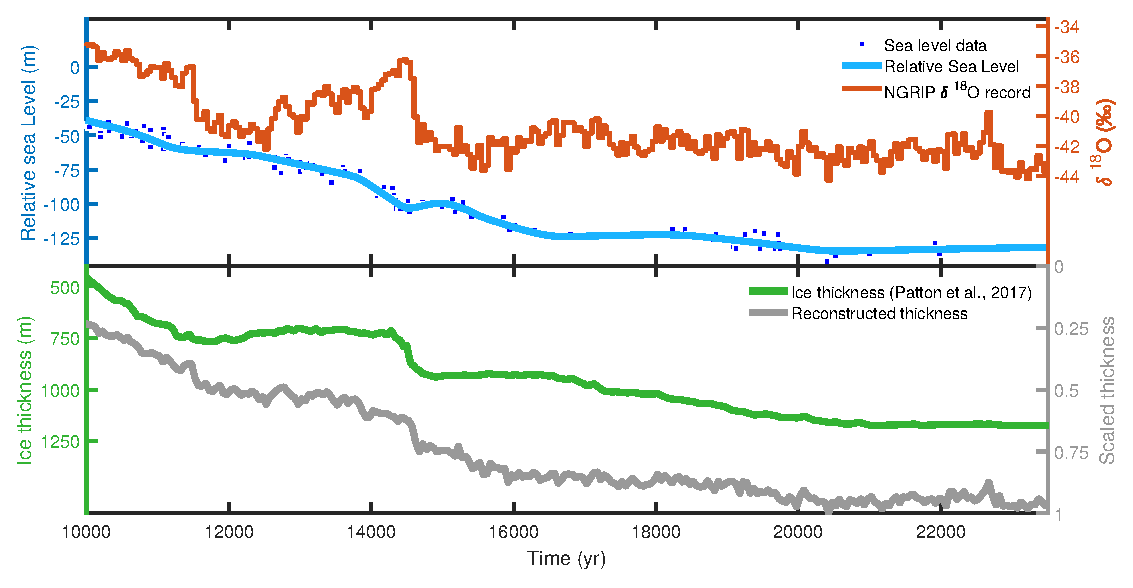
\includegraphics{../figures/version05/supp-figure1.eps}
\caption{We use the NGRIP $\delta^{18}$O, relative sea level history \citep{spratt-2016}, and ice thickness results \citep{lambeck-etal-2014} to create a scaled thickness of the Icelandic Ice Sheet through the deglaciation. Our resultant history tends to preserve some high frequency characteristics of the $\delta^{18}$O record but mutes larger changes such as decrease in ice thickness at the start of the B{\/o}lling-Aller{\/o}d ($\sim$14.7\,ka).}
\label{fg:S1}
\end{figure}

\begin{figure}
\setfigurenum{S2} %%Change number for each figure
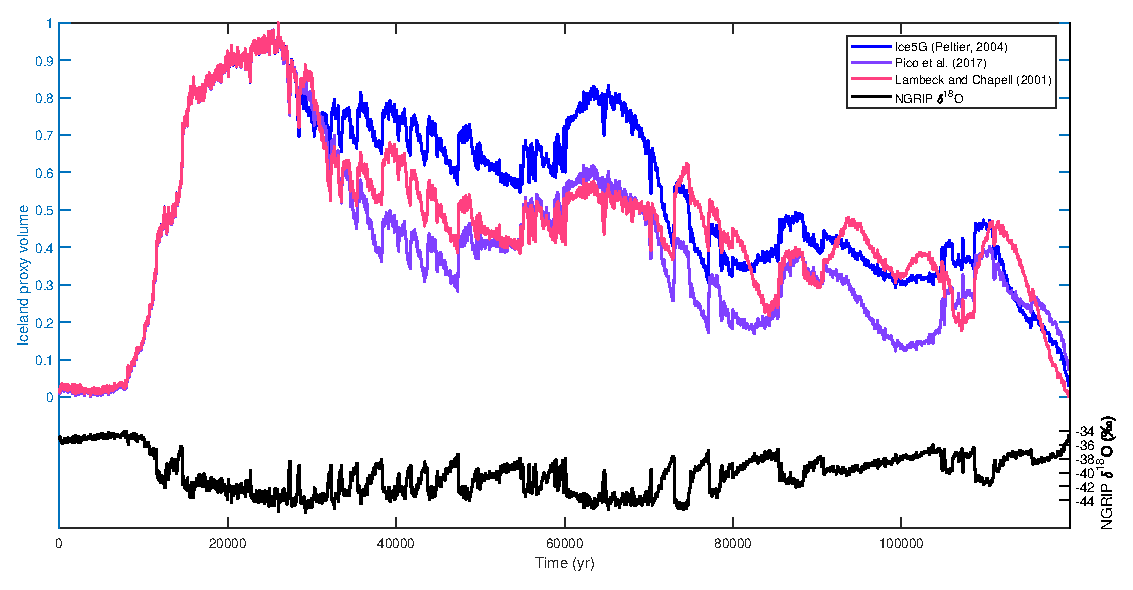
\includegraphics{../figures/version05/supp-figure2.eps}
\caption{Reconstructed ice volumes for 120,000 years to present. Here, we use the differing relative sea level reconstructions \citep{peltier-2004,pico-etal-2017,lambeck-2001} to infer the relative volume of ice in Iceland. The curves match thought the regression period of 10000-23500 years.}
\label{fg:S2}
\end{figure}

\begin{figure}
\setfigurenum{S3}
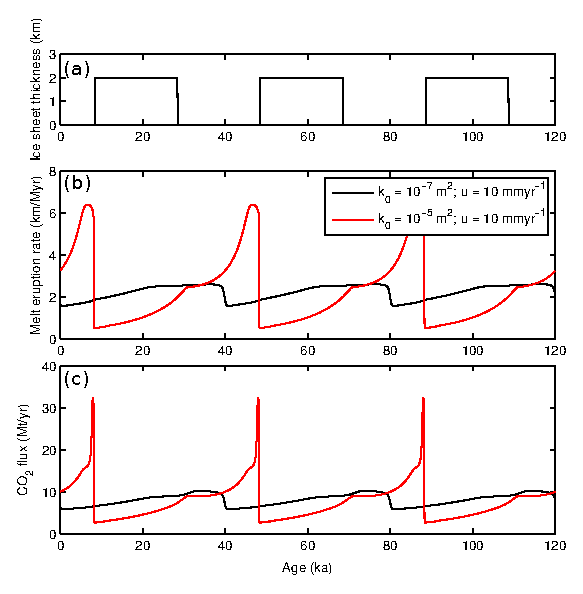
\includegraphics{../figures/version05/supp-figure5.eps}
\caption{Model response to a repeated step change ice sheet thickness. (A) Periodic change in ice sheet thickness assuming a width, $\lambda$, of 200\,km. (B) Model response in terms of eruption rate. Here the model elastic thickness is 10\,km, the viscosity is $10^{21}\rm\,Pa\,s$, the upwelling rate is $10\rm\,mm\,yr^{-1}$, and the mantle temperature is $1450\rm\,^{\circ}C$. The black line is for a permeability coefficient of $10^{-7}\rm\,m^{2}$, and the red line is for a permeability coefficient of $10^{-5}\rm\,m^{2}$. (C) Model response in terms of CO$_{2}$ flux.}
\label{fg:S3}
\end{figure}

\begin{figure}
\setfigurenum{S4}
\includegraphics{../figures/version05/supp-figureN.eps}
\caption{Prediction of melt thickness assuming a mantle temperature of $1450\rm\,^{\circ}C$ and a half spreading rate of $10\rm\,mm\,yr^{-1}$.}
\label{fg:S4}
\end{figure}

% ---------------
% EXAMPLE TABLE
%
%\begin{table}
%\settablenum{S1} %%Change number for each table
%\caption{Time of the Transition Between Phase 1 and Phase 2\tablenotemark{a}}
%\centering
%\begin{tabular}{l c}
%\hline
% Run  & Time (min)  \\
%\hline
%  $l1$  & 260   \\
%  $l2$  & 300   \\
%  $l3$  & 340   \\
%  $h1$  & 270   \\
%  $h2$  & 250   \\
%  $h3$  & 380   \\
%  $r1$  & 370   \\
%  $r2$  & 390   \\
%\hline
%\end{tabular}
%\tablenotetext{a}{Footnote text here.}
%\end{table}
% ---------------
%
% EXAMPLE LARGE TABLE (UPLOADED SEPARATELY)
\begin{table}
\settablenum{S1} %%Change number for each table
\caption{List of model parameters.}
\end{table}


\end{document}
